\scanpage{146}
\figure{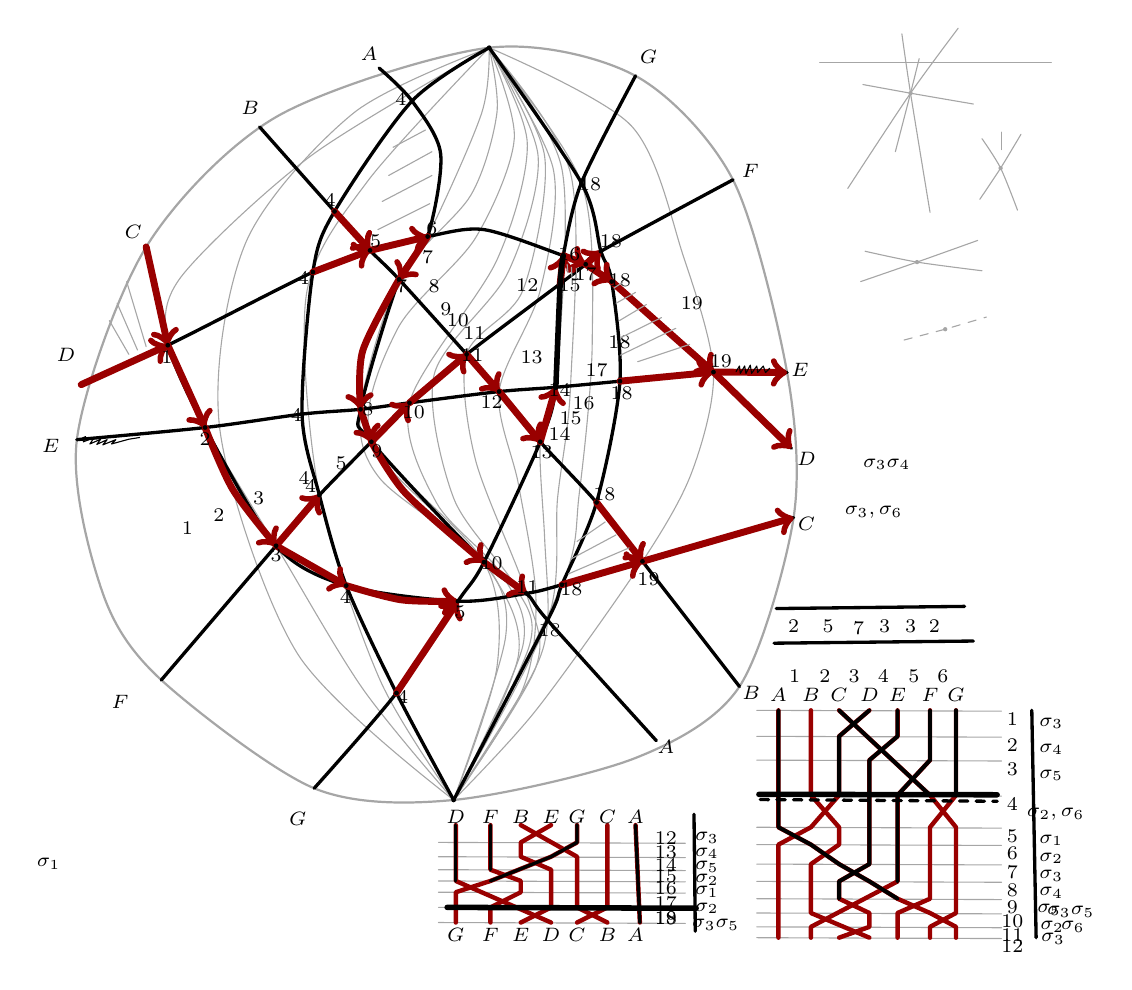
\begin{tikzpicture}[x=.55cm,y=-.55cm,line cap=round,line join=round,g/.style={olive!80!yellow,line width=1.7pt},r/.style={orange!80!brown,line width=1.8pt},w/.style={red!60!black,line width=1.5pt},b/.style={blue!60!black,line width=1.4pt},p/.style={gray!70,thin},k/.style={black,line width=1.2pt},every node/.style={font=\scriptsize}]
% Main large oval and pencil family; individual numbered intersections are retained.
\draw[p,line width=.8pt] plot[smooth cycle] coordinates {(15.92,1.7) (11.0,3.3) (8.0,6.3) (6.4,10.75) (7.0,14.3) (8.35,16.3) (11.88,18.8) (15.1,19.07) (19.3,18.1) (21.7,16.45) (22.95,12.55) (22.8,9.2) (21.55,4.75) (19.3,2.35)};
\draw[p] plot[smooth] coordinates {(15.92,1.7) (12.8,3.2) (10.3,6.2) (9.7,10.5) (11.5,15.7) (15.1,19.07)};
\draw[p] plot[smooth] coordinates {(15.92,1.7) (11.8,4.2) (8.8,7.0) (8.5,8.57) (9.36,10.47) (11.0,13.2) (13.0,16.5) (15.1,19.07)};
\draw[p] plot[smooth] coordinates {(15.92,1.7) (13.1,4.8) (11.7,7.4) (12.0,12.03) (13.4,16.3) (15.1,19.07)};
\draw[p] plot[smooth] coordinates {(15.92,1.7) (15.75,3.2) (14.5,6.06) (13.0,8.8) (13.2,10.8) (15.8,13.58) (16.1,16.0) (15.1,19.07)};
\draw[p] plot[smooth] coordinates {(15.92,1.7) (16.1,3.2) (15.5,5.1) (13.84,7.05) (12.95,10.05) (13.4,11.65) (15.8,13.58) (16.3,15.3) (15.1,19.07)};
\draw[p] plot[smooth] coordinates {(15.92,1.7) (16.5,3.8) (15.6,6.1) (13.8,8.2) (13.2,10.8) (15.8,13.58) (16.6,15.7) (15.1,19.07)};
\draw[p] plot[smooth] coordinates {(15.92,1.7) (16.8,3.9) (16.1,6.6) (14.08,9.9) (14.7,12.2) (16.2,13.85) (16.7,15.5) (15.1,19.07)};
\draw[p] plot[smooth] coordinates {(15.92,1.7) (17.05,4.2) (16.35,6.9) (14.65,9.25) (15.1,12.1) (16.5,14.1) (16.85,15.5) (15.1,19.07)};
\draw[p] plot[smooth] coordinates {(15.92,1.7) (17.2,4.2) (16.7,7.3) (15.4,8.78) (15.6,11.2) (16.78,14.3) (17.0,16.0) (15.1,19.07)};
\draw[p] plot[smooth] coordinates {(15.92,1.7) (17.4,4.5) (17.1,7.3) (16.15,9.64) (16.6,11.8) (17.0,14.4) (16.7,16.5) (15.1,19.07)};
\draw[p] plot[smooth] coordinates {(15.92,1.7) (17.6,4.5) (17.46,9.54) (17.1,10.8) (17.2,13.0) (17.27,14.92) (16.9,16.2) (15.1,19.07)};
\draw[p] plot[smooth] coordinates {(15.92,1.7) (17.8,4.6) (17.8,9.5) (17.5,12.1) (17.27,14.92) (15.1,19.07)};
\draw[p] plot[smooth] coordinates {(15.92,1.7) (18.05,4.82) (18.3,8.5) (18.0,12.0) (17.6,14.1) (15.1,19.07)};
\draw[p] plot[smooth] coordinates {(15.92,1.7) (19.2,3.5) (20.4,6.5) (21.1,9.19) (20.6,11.5) (19.46,13.56) (17.0,17.0) (15.1,19.07)};
\draw[k] plot[smooth] coordinates {(15.92,1.7) (14.14,2.93) (12.35,5.48) (11.85,6.88) (11.6,10.16) (12.0,12.03) (12.62,14.12) (13.78,16.6) (15.1,19.07)};
\draw[k] plot[smooth] coordinates {(15.92,1.7) (18.05,4.82) (18.5,6.4) (18.75,7.1) (18.94,9.4) (18.4,12.2) (17.6,14.1) (17.27,14.92) (15.1,19.07)};
\draw[k] plot[smooth] coordinates {(13.38,2.17) (14.14,2.93) (14.8,4.15) (14.5,6.06) (13.84,7.05) (12.95,10.05) (13.2,10.8) (15.8,13.58) (16.78,14.3) (17.27,14.92) (19.78,17.7)};
\draw[k] plot[smooth] coordinates {(10.62,3.53) (12.35,5.48) (13.17,6.38) (13.84,7.05) (15.4,8.78) (16.15,9.64) (17.1,10.8) (18.4,12.2) (19.46,13.56) (21.7,16.45)};
\draw[k] plot[smooth] coordinates {(8.0,6.3) (8.5,8.57) (9.36,10.47) (11.0,13.2) (12.62,14.12) (15.2,14.48) (16.78,14.3) (17.6,14.1) (19.46,13.56) (22.95,12.55)};
\draw[k] plot[smooth] coordinates {(6.5,9.48) (8.5,8.57) (11.85,6.88) (13.17,6.38) (14.5,6.06) (15.8,5.9) (17.63,6.5) (18.15,6.7) (18.75,7.1) (21.1,9.19) (22.9,10.95)};
\draw[k] plot[smooth] coordinates {(6.4,10.75) (9.36,10.47) (11.6,10.16) (12.95,10.05) (14.08,9.9) (16.15,9.64) (17.46,9.54) (18.94,9.4) (21.1,9.19) (22.8,9.2)};
\draw[k] plot[smooth] coordinates {(8.35,16.3) (11.0,13.2) (12.0,12.03) (13.2,10.8) (14.08,9.9) (15.4,8.78) (17.56,7.15) (18.15,6.7) (18.5,6.4) (21.55,4.75)};
\draw[k] plot[smooth] coordinates {(11.88,18.8) (13.78,16.6) (15.2,14.48) (15.8,13.58) (17.1,10.8) (17.46,9.54) (17.56,7.15) (17.63,6.5) (18.05,4.82) (19.3,2.35)};
\draw[w,->,line width=2.5pt] plot[smooth] coordinates {(8.0,6.3) (8.5,8.57)};
\draw[w,->,line width=2.5pt] plot[smooth] coordinates {(6.5,9.48) (8.5,8.57)};
\draw[w,->,line width=2.5pt] plot[smooth] coordinates {(8.5,8.57) (9.36,10.47)};
\draw[w,->,line width=2.5pt] plot[smooth] coordinates {(9.36,10.47) (10.0,11.9) (11.0,13.2)};
\draw[w,->,line width=2.5pt] plot[smooth] coordinates {(11.0,13.2) (12.0,12.03)};
\draw[w,->,line width=2.5pt] plot[smooth] coordinates {(11.0,13.2) (12.62,14.12)};
\draw[w,->,line width=2.5pt] plot[smooth] coordinates {(12.62,14.12) (13.9,14.45) (15.2,14.48)};
\draw[w,->,line width=2.5pt] plot[smooth] coordinates {(13.78,16.6) (15.2,14.48)};
\draw[w,->,line width=2.5pt] plot[smooth] coordinates {(12.35,5.48) (13.17,6.38)};
\draw[w,->,line width=2.5pt] plot[smooth] coordinates {(11.85,6.88) (13.17,6.38)};
\draw[w,->,line width=2.5pt] plot[smooth] coordinates {(13.17,6.38) (14.5,6.06)};
\draw[w,->,line width=2.5pt] plot[smooth] coordinates {(14.5,6.06) (13.84,7.05)};
\draw[w,->,line width=2.5pt] plot[smooth] coordinates {(13.84,7.05) (13.0,8.7) (12.95,10.05)};
\draw[w,->,line width=2.5pt] plot[smooth] coordinates {(12.95,10.05) (13.2,10.8)};
\draw[w,->,line width=2.5pt] plot[smooth] coordinates {(13.2,10.8) (14.08,9.9)};
\draw[w,->,line width=2.5pt] plot[smooth] coordinates {(14.08,9.9) (15.4,8.78)};
\draw[w,->,line width=2.5pt] plot[smooth] coordinates {(15.4,8.78) (16.15,9.64)};
\draw[w,->,line width=2.5pt] plot[smooth] coordinates {(16.15,9.64) (17.1,10.8)};
\draw[w,->,line width=2.5pt] plot[smooth] coordinates {(17.1,10.8) (17.46,9.54)};
\draw[w,->,line width=2.5pt] plot[smooth] coordinates {(13.2,10.8) (14.0,12.0) (15.8,13.58)};
\draw[w,->,line width=2.5pt] plot[smooth] coordinates {(15.8,13.58) (16.78,14.3)};
\draw[w,->,line width=2.5pt] plot[smooth] coordinates {(17.6,14.1) (19.46,13.56)};
\draw[w,->,line width=2.5pt] plot[smooth] coordinates {(18.4,12.2) (19.46,13.56)};
\draw[w,->,line width=2.5pt] plot[smooth] coordinates {(19.46,13.56) (22.95,12.55)};
\draw[w,->,line width=2.5pt] plot[smooth] coordinates {(17.56,7.15) (17.63,6.5)};
\draw[w,->,line width=2.5pt] plot[smooth] coordinates {(17.63,6.5) (18.15,6.7)};
\draw[w,->,line width=2.5pt] plot[smooth] coordinates {(18.15,6.7) (18.5,6.4)};
\draw[w,->,line width=2.5pt] plot[smooth] coordinates {(18.15,6.7) (18.75,7.1)};
\draw[w,->,line width=2.5pt] plot[smooth] coordinates {(18.75,7.1) (21.1,9.19)};
\draw[w,->,line width=2.5pt] plot[smooth] coordinates {(18.94,9.4) (21.1,9.19)};
\draw[w,->,line width=2.5pt] plot[smooth] coordinates {(21.1,9.19) (22.8,9.2)};
\draw[w,->,line width=2.5pt] plot[smooth] coordinates {(21.1,9.19) (22.9,10.95)};
\draw[k,line width=2pt] plot[smooth] coordinates {(17.46,9.54) (17.56,7.15) (17.63,6.5)};
\fill[k] (15.92,1.7) circle (.055);
\fill[k] (15.1,19.07) circle (.055);
\fill[k] (14.14,2.93) circle (.055);
\fill[k] (12.35,5.48) circle (.055);
\fill[k] (11.85,6.88) circle (.055);
\fill[k] (11.6,10.16) circle (.055);
\fill[k] (12.0,12.03) circle (.055);
\fill[k] (12.62,14.12) circle (.055);
\fill[k] (13.78,16.6) circle (.055);
\fill[k] (18.05,4.82) circle (.055);
\fill[k] (18.5,6.4) circle (.055);
\fill[k] (18.75,7.1) circle (.055);
\fill[k] (18.94,9.4) circle (.055);
\fill[k] (18.4,12.2) circle (.055);
\fill[k] (17.6,14.1) circle (.055);
\fill[k] (17.27,14.92) circle (.055);
\fill[k] (14.5,6.06) circle (.055);
\fill[k] (13.84,7.05) circle (.055);
\fill[k] (12.95,10.05) circle (.055);
\fill[k] (13.2,10.8) circle (.055);
\fill[k] (15.8,13.58) circle (.055);
\fill[k] (16.78,14.3) circle (.055);
\fill[k] (13.17,6.38) circle (.055);
\fill[k] (15.4,8.78) circle (.055);
\fill[k] (16.15,9.64) circle (.055);
\fill[k] (17.1,10.8) circle (.055);
\fill[k] (19.46,13.56) circle (.055);
\fill[k] (8.5,8.57) circle (.055);
\fill[k] (9.36,10.47) circle (.055);
\fill[k] (11.0,13.2) circle (.055);
\fill[k] (15.2,14.48) circle (.055);
\fill[k] (17.63,6.5) circle (.055);
\fill[k] (18.15,6.7) circle (.055);
\fill[k] (21.1,9.19) circle (.055);
\fill[k] (14.08,9.9) circle (.055);
\fill[k] (17.46,9.54) circle (.055);
\fill[k] (17.56,7.15) circle (.055);
\node at (13.15,1.85) {$A$};
\node at (10.4,3.1) {$B$};
\node at (7.7,5.95) {$C$};
\node at (6.15,8.8) {$D$};
\node at (5.8,10.9) {$E$};
\node at (7.4,16.8) {$F$};
\node at (11.5,19.5) {$G$};
\node at (19.6,1.92) {$G$};
\node at (21.95,4.55) {$F$};
\node at (23.1,9.15) {$E$};
\node at (23.25,11.2) {$D$};
\node at (23.25,12.7) {$C$};
\node at (21.97,16.6) {$B$};
\node at (20.0,17.85) {$A$};
\node at (5.75,20.55) {$\sigma_1$};
\node at (8.48,8.85) {$1$};
\node at (9.36,10.73) {$2$};
\node at (11.0,13.43) {$3$};
\node at (12.6,14.38) {$4$};
\node at (15.25,14.73) {$5$};
\node at (14.6,5.88) {$6$};
\node at (13.9,7.2) {$7$};
\node at (13.12,10.05) {$8$};
\node at (13.33,11.02) {$9$};
\node at (14.18,10.12) {$10$};
\node at (15.53,8.8) {$11$};
\node at (15.98,9.88) {$12$};
\node at (17.13,11.03) {$13$};
\node at (17.55,9.6) {$14$};
\node at (17.78,7.18) {$15$};
\node at (17.77,6.47) {$16$};
\node at (18.15,6.94) {$17$};
\node at (18.73,6.17) {$18$};
\node at (18.94,7.07) {$18$};
\node at (18.98,9.68) {$18$};
\node at (18.58,12.0) {$18$};
\node at (17.82,14.2) {$18$};
\node at (17.32,15.15) {$18$};
\node at (18.25,4.85) {$18$};
\node at (21.27,8.95) {$19$};
\node at (19.6,13.98) {$19$};
\node at (15.98,13.6) {$10$};
\node at (16.8,14.16) {$11$};
\node at (13.92,16.7) {$4$};
\node at (12.25,5.23) {$4$};
\node at (11.63,7.02) {$4$};
\node at (11.47,10.18) {$4$};
\node at (11.8,11.83) {$4$};
\node at (13.3,6.17) {$5$};
\node at (13.88,2.88) {$4$};
\node at (8.95,12.8) {$1$};
\node at (9.68,12.5) {$2$};
\node at (10.6,12.1) {$3$};
\node at (11.65,11.65) {$4$};
\node at (12.5,11.3) {$5$};
\node at (14.5,6.53) {$7$};
\node at (14.65,7.2) {$8$};
\node at (14.92,7.75) {$9$};
\node at (15.2,8.0) {$10$};
\node at (15.58,8.3) {$11$};
\node at (16.8,7.18) {$12$};
\node at (16.9,8.85) {$\unsure{13}$};
\node at (17.55,10.63) {$14$};
\node at (17.8,10.25) {$15$};
\node at (18.1,9.9) {$16$};
\node at (18.4,9.15) {$17$};
\node at (18.93,8.5) {$18$};
\node at (20.6,7.6) {$19$};
\draw[p,thin] (7.15,8.0)--(7.6,8.78);
\draw[p,thin] (7.33,7.6)--(7.8,8.68);
\draw[p,thin] (7.55,7.1)--(8.0,8.6);
\draw[p,thin] (13.7,4.0)--(14.45,3.6);
\draw[p,thin] (13.6,4.65)--(14.6,4.1);
\draw[p,thin] (13.45,5.25)--(14.6,4.65);
\draw[p,thin] (13.35,5.9)--(14.55,5.3);
\draw[p,thin] (17.72,6.7)--(17.74,6.9);
\draw[p,thin] (17.82,6.77)--(17.83,6.98);
\draw[p,thin] (17.93,6.81)--(17.93,7.02);
\draw[p,thin] (18.8,7.25)--(19.0,7.12);
\draw[p,thin] (18.85,7.6)--(19.3,7.35);
\draw[p,thin] (18.93,8.0)--(19.55,7.63);
\draw[p,thin] (18.95,8.4)--(19.9,7.93);
\draw[p,thin] (18.95,8.8)--(20.23,8.18);
\draw[p,thin] (19.35,8.95)--(20.55,8.55);
\draw[p,thin] (17.95,13.1)--(18.6,12.65);
\draw[p,thin] (17.82,13.5)--(18.85,12.95);
\draw[p,thin] (17.75,13.85)--(19.15,13.25);
\draw[k,thin] (6.45,10.75)--(6.6,10.68)--(6.55,10.8)--(6.8,10.7)--(6.7,10.85)--(6.95,10.74)--(6.86,10.86)--(7.1,10.75)--(7.0,10.87)--(7.3,10.75)--(7.2,10.85)--(7.6,10.74)--(7.85,10.7);
\draw[k,thin] (21.62,9.18)--(21.7,9.05)--(21.72,9.22)--(21.82,9.05)--(21.85,9.22)--(21.95,9.03)--(21.98,9.22)--(22.1,9.05)--(22.12,9.2)--(22.25,9.05)--(22.3,9.2)--(22.4,9.1);
% Small right-hand sketches and cancelled symbols.
\draw[p] plot[smooth] coordinates {(23.55,2.05) (28.9,2.05)};
\draw[p] plot[smooth] coordinates {(25.45,1.38) (25.65,2.75) (26.1,5.5)};
\draw[p] plot[smooth] coordinates {(24.2,4.95) (25.65,2.75) (26.75,1.25)};
\draw[p] plot[smooth] coordinates {(24.55,2.55) (25.65,2.75) (27.1,3.0)};
\draw[p] plot[smooth] coordinates {(25.3,4.1) (25.65,2.75) (25.85,1.95)};
\draw[p] plot[smooth] coordinates {(27.3,3.8) (27.73,4.48) (28.12,5.45)};
\draw[p] plot[smooth] coordinates {(28.2,3.7) (27.73,4.48) (27.25,5.2)};
\draw[p] plot[smooth] coordinates {(27.75,3.65) (27.75,4.05)};
\draw[p] plot[smooth] coordinates {(24.5,7.1) (25.8,6.65) (27.2,6.15)};
\draw[p] plot[smooth] coordinates {(24.6,6.4) (25.8,6.65) (27.3,6.85)};
\draw[p,dashed] (25.5,8.45)--(26.45,8.2)--(27.4,7.92);
\fill[p] (25.65,2.75) circle (.05);
\fill[p] (27.73,4.48) circle (.05);
\fill[p] (25.8,6.65) circle (.05);
\fill[p] (26.45,8.2) circle (.05);
\node at (25.1,11.32) {$\deleted{\unsure{\sigma_3\sigma_4}}$};
\node at (24.8,12.43) {$\deleted{\unsure{\sigma_3,\sigma_6}}$};
\draw[k] (22.55,14.65)--(26.9,14.6);
\draw[k] (22.5,15.45)--(27.1,15.4);
\node at (22.95,15.07) {$2$};
\node at (23.75,15.05) {$5$};
\node at (24.45,15.1) {$7$};
\node at (25.05,15.05) {$3$};
\node at (25.65,15.05) {$3$};
\node at (26.2,15.05) {$2$};
% Lower-right strand grid, rows 1 to 12.
\draw[p] (22.1,17.0)--(27.75,17.02);
\node at (28.0,17.2) {$1$};
\draw[p] (22.1,17.6)--(27.75,17.62);
\node at (28.0,17.8) {$2$};
\draw[p] (22.1,18.15)--(27.75,18.169999999999998);
\node at (28.0,18.349999999999998) {$3$};
\draw[p] (22.1,18.96)--(27.75,18.98);
\node at (28.0,19.16) {$4$};
\draw[p] (22.1,19.7)--(27.75,19.72);
\node at (28.0,19.9) {$5$};
\draw[p] (22.1,20.1)--(27.75,20.12);
\node at (28.0,20.3) {$6$};
\draw[p] (22.1,20.55)--(27.75,20.57);
\node at (28.0,20.75) {$7$};
\draw[p] (22.1,20.95)--(27.75,20.97);
\node at (28.0,21.15) {$8$};
\draw[p] (22.1,21.35)--(27.75,21.37);
\node at (28.0,21.55) {$9$};
\draw[p] (22.1,21.68)--(27.75,21.7);
\node at (28.0,21.88) {$10$};
\draw[p] (22.1,22.0)--(27.75,22.02);
\node at (28.0,22.2) {$11$};
\draw[p] (22.1,22.25)--(27.75,22.27);
\node at (28.0,22.45) {$12$};
\draw[w,line width=1.6pt] (22.6,17.0)--(22.6,19.7)--(23.35,20.1)--(24.0,20.55)--(24.7,20.95)--(25.35,21.35)--(26.1,21.68)--(26.7,22.0)--(26.7,22.25);
\draw[w,line width=1.6pt] (23.35,17.0)--(23.35,18.96)--(24.0,19.7)--(24.0,20.1)--(23.35,20.55)--(23.35,21.68)--(24.7,22.25);
\draw[w,line width=1.6pt] (24.0,17.0)--(26.1,18.96)--(26.7,19.7)--(26.7,21.68)--(26.1,22.0)--(26.1,22.25);
\draw[w,line width=1.6pt] (24.7,17.0)--(24.0,17.6)--(24.0,18.96)--(23.35,19.7)--(22.6,20.1)--(22.6,22.25);
\draw[w,line width=1.6pt] (25.35,17.0)--(25.35,17.6)--(24.7,18.15)--(24.7,20.55)--(24.0,20.95)--(24.0,21.35)--(24.7,21.68)--(24.7,22.0)--(24.0,22.25);
\draw[w,line width=1.6pt] (26.1,17.0)--(26.1,18.15)--(25.35,18.96)--(25.35,20.95)--(23.35,22.0)--(23.35,22.25);
\draw[w,line width=1.6pt] (26.7,17.0)--(26.7,18.96)--(26.1,19.7)--(26.1,21.35)--(25.35,21.68)--(25.35,22.25);
\draw[k,line width=1.4pt] (22.6,17.0)--(22.6,19.7)--(23.35,20.1)--(24.0,20.55)--(24.7,20.95)--(25.35,21.35);
\draw[k,line width=1.4pt] (24.0,17.0)--(26.1,18.96);
\draw[k,line width=1.4pt] (24.7,17.0)--(24.0,17.6)--(24.0,18.96);
\draw[k,line width=1.4pt] (25.35,17.0)--(25.35,17.6)--(24.7,18.15)--(24.7,20.55)--(24.0,20.95)--(24.0,21.35);
\draw[k,line width=1.4pt] (26.1,17.0)--(26.1,18.15)--(25.35,18.96)--(25.35,20.95);
\draw[k,line width=1.4pt] (26.7,17.0)--(26.7,18.96);
\draw[k,line width=2pt] (22.15,18.94)--(27.65,18.95);
\draw[k,dashed] (22.18,19.06)--(27.65,19.1);
\node at (22.6,16.65) {$A$};
\node at (23.35,16.65) {$B$};
\node at (24.0,16.65) {$C$};
\node at (24.7,16.65) {$D$};
\node at (25.35,16.65) {$E$};
\node at (26.1,16.65) {$F$};
\node at (26.7,16.65) {$G$};
\node at (22.975,16.22) {$1$};
\node at (23.675,16.22) {$2$};
\node at (24.35,16.22) {$3$};
\node at (25.025,16.22) {$4$};
\node at (25.725,16.22) {$5$};
\node at (26.4,16.22) {$6$};
\draw[k] (28.45,17.0)--(28.55,22.25);
\node at (28.9,17.3) {$\sigma_3$};
\node at (28.9,17.9) {$\sigma_4$};
\node at (28.9,18.5) {$\sigma_5$};
\node at (29.0,19.4) {$\sigma_2,\sigma_6$};
\node at (28.9,20.0) {$\sigma_1$};
\node at (28.9,20.42) {$\sigma_2$};
\node at (28.9,20.82) {$\sigma_3$};
\node at (28.9,21.22) {$\sigma_4$};
\node at (28.85,21.6) {$\deleted{\unsure{\sigma_5}}$};
\node at (29.35,21.65) {$\unsure{\sigma_3\sigma_5}$};
\node at (28.92,22.0) {$\sigma_2$};
\node at (29.4,22.0) {$\unsure{\sigma_6}$};
\node at (28.94,22.28) {$\unsure{\sigma_3}$};
% Lower central continuation grid, with its own written upper order.
\draw[p] (14.75,20.05)--(20.45,20.07);
\node at (20.0,19.95) {$12$};
\draw[p] (14.75,20.38)--(20.45,20.4);
\node at (20.0,20.279999999999998) {$13$};
\draw[p] (14.75,20.68)--(20.45,20.7);
\node at (20.0,20.58) {$14$};
\draw[p] (14.75,20.94)--(20.45,20.96);
\node at (20.0,20.84) {$15$};
\draw[p] (14.75,21.2)--(20.45,21.22);
\node at (20.0,21.099999999999998) {$16$};
\draw[p] (14.75,21.55)--(20.45,21.57);
\node at (20.0,21.45) {$17$};
\draw[p] (14.75,21.9)--(20.45,21.919999999999998);
\node at (20.0,21.799999999999997) {$18$};
\draw[w,line width=1.6pt] (15.15,19.65)--(15.15,20.94)--(17.35,21.9);
\draw[w,line width=1.6pt] (15.95,19.65)--(15.95,20.68)--(16.65,20.94)--(16.65,21.2)--(15.95,21.55)--(15.95,21.9);
\draw[w,line width=1.6pt] (16.65,19.65)--(17.95,20.38)--(17.95,21.55)--(18.65,21.9);
\draw[w,line width=1.6pt] (17.35,19.65)--(16.65,20.05)--(16.65,20.38)--(17.35,20.68)--(17.35,21.55)--(16.65,21.9);
\draw[w,line width=1.6pt] (17.95,19.65)--(17.95,20.05)--(17.35,20.38)--(15.95,20.94)--(15.15,21.2)--(15.15,21.9);
\draw[w,line width=1.6pt] (18.65,19.65)--(18.65,21.55)--(17.95,21.9);
\draw[w,line width=1.6pt] (19.3,19.65)--(19.4,21.9);
\draw[k] (15.15,19.65)--(15.15,20.94);
\draw[k] (15.95,19.65)--(15.95,20.68);
\draw[k] (17.95,19.65)--(17.95,20.05)--(17.35,20.38)--(15.95,20.94);
\draw[k] (19.3,19.65)--(19.4,21.9);
\draw[k,line width=2pt] (14.95,21.55)--(20.7,21.57);
\draw[k] (20.65,19.4)--(20.68,22.1);
\node at (15.15,19.45) {$D$};
\node at (15.95,19.45) {$F$};
\node at (16.65,19.45) {$B$};
\node at (17.35,19.45) {$E$};
\node at (17.95,19.45) {$G$};
\node at (18.65,19.45) {$C$};
\node at (19.3,19.45) {$A$};
\node at (15.15,22.18) {$G$};
\node at (15.95,22.18) {$F$};
\node at (16.65,22.18) {$E$};
\node at (17.35,22.18) {$D$};
\node at (17.95,22.18) {$C$};
\node at (18.65,22.18) {$B$};
\node at (19.3,22.18) {$A$};
\node at (20.95,19.95) {$\sigma_3$};
\node at (20.95,20.3) {$\sigma_4$};
\node at (20.95,20.62) {$\sigma_5$};
\node at (20.95,20.91) {$\deleted{\unsure{\sigma_2}}$};
\node at (20.95,21.2) {$\sigma_1$};
\node at (20.95,21.57) {$\sigma_2$};
\node at (20.0,21.8) {$\unsure{19}$};
\node at (21.15,21.95) {$\sigma_3\sigma_5$};
\end{tikzpicture}}
{\color{gray}\scriptsize\unsure{\begin{tabular}{l}
\texttt{\ \ \ \ \ \ \ \ \ \ \ 00000000\ \ \ \ \ \ 00000000\ \ \ \ \ \ 00000000\ \ \ \ \ \ 00000000}\\
\texttt{\ \ \ \ \ \ \ \ \ 0000000000\ \ \ \ 0000000000\ \ \ \ 0000000000\ \ \ \ 0000000000}\\
\texttt{\ \ \ \ \ \ \ 00\ \ \ \ \ \ 0000\ \ 00\ \ \ \ \ \ 0000\ \ 00\ \ \ \ \ \ 0000\ \ 00\ \ \ \ \ \ 0000}\\
\texttt{\ \ \ \ \ \ 00\ \ \ \ \ 00\ 00\ \ 00\ \ \ \ \ 00\ 00\ \ 00\ \ \ \ \ 00\ 00\ \ 00\ \ \ \ \ 00\ 00}\\
\texttt{\ \ \ \ \ 00\ \ \ \ 00\ \ 00\ \ 00\ \ \ \ 00\ \ 00\ \ 00\ \ \ \ 00\ \ 00\ \ 00\ \ \ \ 00\ \ 00}\\
\texttt{\ \ \ \ 00\ \ \ 00\ \ \ 00\ \ 00\ \ \ 00\ \ \ 00\ \ 00\ \ \ 00\ \ \ 00\ \ 00\ \ \ 00\ \ \ 00}\\
\texttt{\ \ \ 00\ \ 00\ \ \ \ 00\ \ 00\ \ 00\ \ \ \ 00\ \ 00\ \ 00\ \ \ \ 00\ \ 00\ \ 00\ \ \ \ 00}\\
\texttt{\ \ 00\ 00\ \ \ \ \ 00\ \ 00\ 00\ \ \ \ \ 00\ \ 00\ 00\ \ \ \ \ 00\ \ 00\ 00\ \ \ \ \ 00}\\
\texttt{\ 0000\ \ \ \ \ \ 00\ \ 0000\ \ \ \ \ \ 00\ \ 0000\ \ \ \ \ \ 00\ \ 0000\ \ \ \ \ \ 00}\\
\texttt{000\ \ \ \ \ \ \ 00\ \ 000\ \ \ \ \ \ \ 00\ \ 000\ \ \ \ \ \ \ 00\ \ 000\ \ \ \ \ \ \ 00}\\
\texttt{0000000000\ \ \ \ 0000000000\ \ \ \ 0000000000\ \ \ \ 0000000000}\\
\texttt{00000000\ \ \ \ \ \ 00000000\ \ \ \ \ \ 00000000\ \ \ \ \ \ 00000000}\\
\texttt{}\\
\texttt{\ CCCCCCCCCC\ \ \ RRRRRRRRRRR\ \ \ AAAAAAAAAA\ \ \ YY\ \ \ \ \ \ \ \ YY\ \ \ 2222222222}\\
\texttt{CCCCCCCCCCCC\ \ RRRRRRRRRRRR\ AAAAAAAAAAAA\ \ YY\ \ \ \ \ \ \ \ YY\ \ 222222222222}\\
\texttt{CC\ \ \ \ \ \ \ \ CC\ \ RR\ \ \ \ \ \ \ \ RR\ AA\ \ \ \ \ \ \ \ AA\ \ YY\ \ \ \ \ \ YY\ \ \ 22\ \ \ \ \ \ \ \ 22}\\
\texttt{CC\ \ \ \ \ \ \ \ \ \ \ \ RR\ \ \ \ \ \ \ \ RR\ AA\ \ \ \ \ \ \ \ AA\ \ \ YY\ \ \ \ YY\ \ \ \ \ \ \ \ \ \ \ \ \ 22}\\
\texttt{CC\ \ \ \ \ \ \ \ \ \ \ \ RR\ \ \ \ \ \ \ \ RR\ AA\ \ \ \ \ \ \ \ AA\ \ \ \ YY\ \ YY\ \ \ \ \ \ \ \ \ \ \ \ \ \ 22}\\
\texttt{CC\ \ \ \ \ \ \ \ \ \ \ \ RRRRRRRRRRRR\ AAAAAAAAAAAA\ \ \ \ \ YYYY\ \ \ \ \ \ \ \ \ \ \ \ \ \ 22}\\
\texttt{CC\ \ \ \ \ \ \ \ \ \ \ \ RRRRRRRRRRR\ \ AAAAAAAAAAAA\ \ \ \ \ \ YY\ \ \ \ \ \ \ \ \ \ \ \ \ \ 22}\\
\texttt{CC\ \ \ \ \ \ \ \ \ \ \ \ RR\ \ \ \ RR\ \ \ \ \ AA\ \ \ \ \ \ \ \ AA\ \ \ \ \ \ YY\ \ \ \ \ \ \ \ \ \ \ \ \ 22}\\
\texttt{CC\ \ \ \ \ \ \ \ \ \ \ \ RR\ \ \ \ \ RR\ \ \ \ AA\ \ \ \ \ \ \ \ AA\ \ \ \ \ \ YY\ \ \ \ \ \ \ \ \ \ \ \ 22}\\
\texttt{CC\ \ \ \ \ \ \ \ CC\ \ RR\ \ \ \ \ \ RR\ \ \ AA\ \ \ \ \ \ \ \ AA\ \ \ \ \ \ YY\ \ \ \ \ \ \ \ \ \ \ 22}\\
\texttt{CCCCCCCCCCCC\ \ RR\ \ \ \ \ \ \ RR\ \ AA\ \ \ \ \ \ \ \ AA\ \ \ \ \ \ YY\ \ \ \ \ \ \ \ \ \ 222222222222}\\
\texttt{\ CCCCCCCCCC\ \ \ RR\ \ \ \ \ \ \ \ RR\ AA\ \ \ \ \ \ \ \ AA\ \ \ \ \ \ YY\ \ \ \ \ \ \ \ \ \ 222222222222}\\
\end{tabular}}}
{\color{gray}\ttfamily\unsure{0025 CRAY2 ***}}
{\color{gray}\ttfamily ****A\quad START\quad JOB\quad25\quad CRAY2\quad ROOM\quad\unsure{9.01.53} AM 19 AUG 82\quad\unsure{R6.PR1}\quad SYS JES2\quad JOB\quad25\quad START\quad A****}\\
{\color{gray}\ttfamily ****A\quad START\quad JOB\quad25\quad CRAY2\quad ROOM\quad\unsure{9.01.53} AM 19 AUG 82\quad\unsure{R6.PR1}\quad SYS JES2\quad JOB\quad25\quad START\quad A****}\\
{\color{gray}\ttfamily ****A\quad START\quad JOB\quad25\quad CRAY2\quad ROOM\quad\unsure{9.01.53} AM 19 AUG 82\quad\unsure{R6.PR1}\quad SYS JES2\quad JOB\quad25\quad START\quad A****}\\
{\color{gray}\ttfamily ****A\quad START\quad JOB\quad25\quad CRAY2\quad ROOM\quad\unsure{9.01.53} AM 19 AUG 82\quad\unsure{R6.PR1}\quad SYS JES2\quad JOB\quad25\quad START\quad A****}\\
{\color{gray}\ttfamily ****A\quad START\quad JOB\quad25\quad CRAY2\quad ROOM\quad\unsure{9.01.53} AM 19 AUG 82\quad\unsure{R6.PR1}\quad SYS JES2\quad JOB\quad25\quad START\quad A****}\\
{\color{gray}\ttfamily ****A\quad START\quad JOB\quad25\quad CRAY2\quad ROOM\quad\unsure{9.01.53|9.01.57} AM 19 AUG 82\quad\unsure{R6.PR1}\quad SYS JES2\quad JOB\quad25\quad START\quad A****}\\
{\color{gray}\ttfamily
DERNIERE MISE A JOUR DE JOURNAL : 11-08-82\\
ATTENTION .........\\
T\quad UN ARRET EXCEPTIONNEL POUR PREPARER L'ARRIVEE \unsure{DE NOUVELLES}\\
T\quad \unsure{UNITES} AURA LIEU DU VENDREDI 20 AOUT A 17H\unsure{30} \unsure{AU LUNDI}\\
T\quad 23 AOUT A 8H.
}
\margin{\mspage{145}}
